\chapter{Results}
\label{chapter:results}

\section{Overview}
This chapter presents the results of the testing done on the three propagation methods, their timings, throughput and speedup against the sequential versions. The CPU used to test the implementation was an Intel(R) Core(TM) i7-3770K CPU @ 3.50GHz. The GPU used was a GTX-970 with 4GB of RAM and 1664 cuda cores. The sequential timings were accomplished without implementing any parallel component on the CPU. 

In order to run a simulation using this library, three files are needed. A .dem file of the region of interest is needed to determine terrain, and all files are required to be in UTM format. The second file needed is a fuel model file that contains the necessary fuel model data needed for a particular simulation. The third file needed is the fuel model file which relates fuel models to cells in the terrain file. In order to run crowning, three additional data files are needed: canopy height, crown base height, and crown bulk density. 

\section{Spread Images}\label{spread_ims}
This section shows the results of the base spread with acceleration integrated for all three methods. The spread patterns produce similar results, but slightly different patterns. The results of the three spread propagations for a flat plane with no wind influence can be seen in Figures \ref{fig:burn_dist} through \ref{fig:it_min_time}.
\begin{figure}%[!b]
\centering
  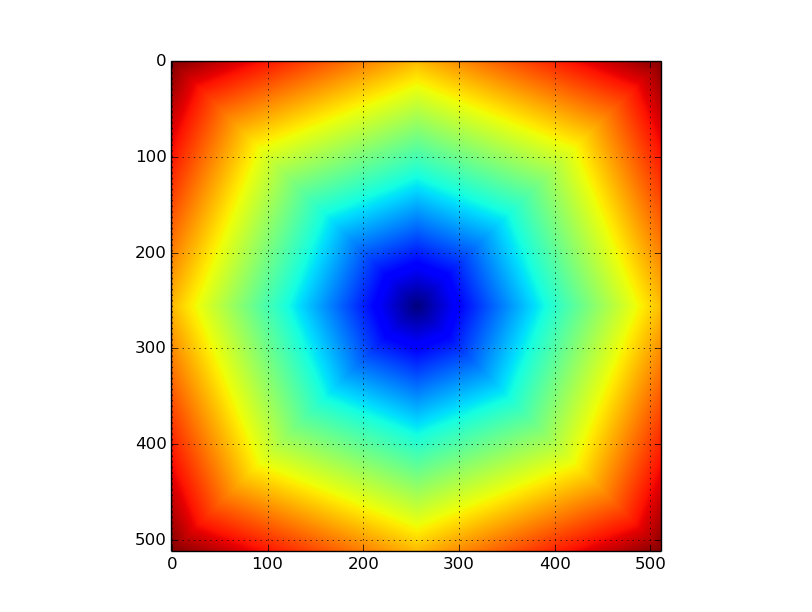
\includegraphics[height=0.27\textheight]{figures/results/burn_dist.png}
  \caption{The Burn Distances Kernel burn pattern at a grid size of 512x512.}
  \label{fig:burn_dist}
\end{figure}
\begin{figure}%[!b]
\centering
  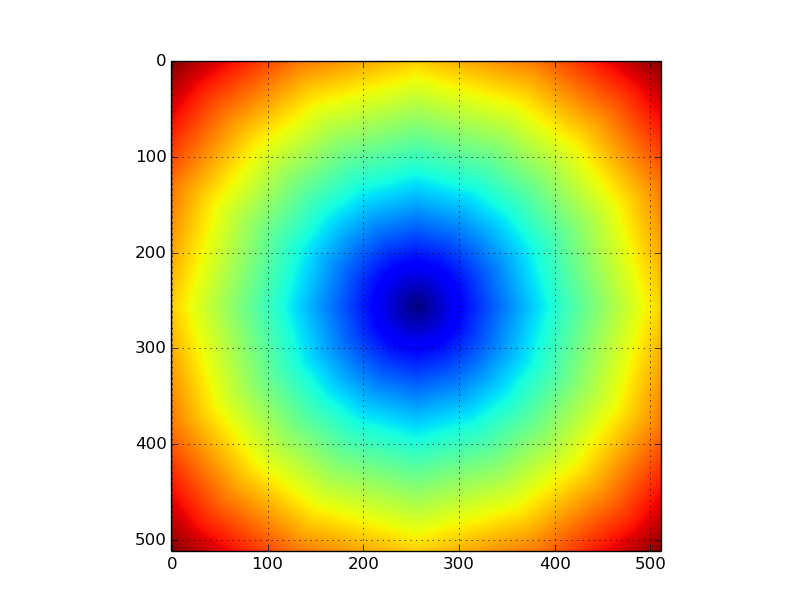
\includegraphics[height=0.27\textheight]{figures/results/min_time.png}
  \caption{The Minimal Time Kernel burn pattern at a grid size of 512x512.}
  \label{fig:min_time}
\end{figure}
\begin{figure}%[!b]
\centering
  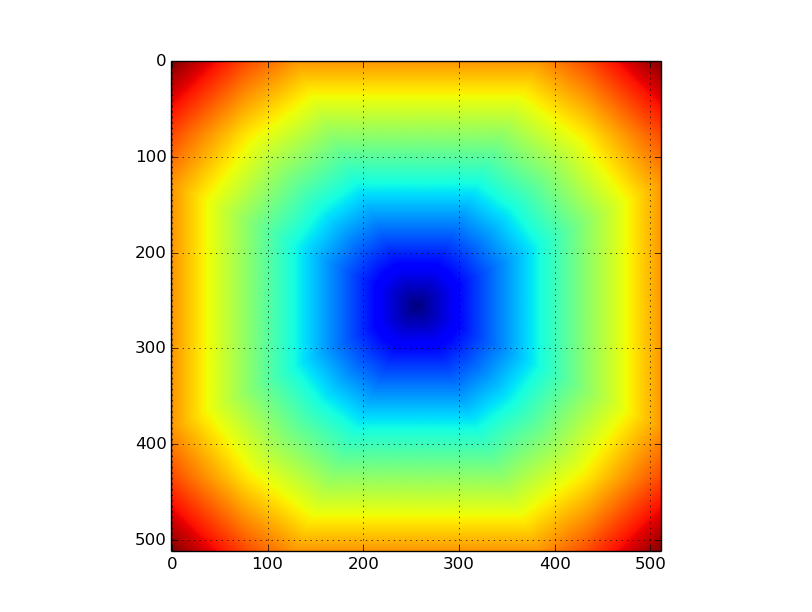
\includegraphics[height=0.27\textheight]{figures/results/it_min_time.png}
  \caption{The Iterative Minimal Time Kernel burn pattern at a grid size of 512x512.}
  \label{fig:it_min_time}
\end{figure}

\section{Running Time Comparison}
This section compares the running times achieved by the different methods. It first compares the effect of adding the crowning behavior to the simulation and its impact on running time and then presents the runtime results of the experiments.

\subsection*{Crowning and Acceleration Time Differences}
This section presents results on the running times for the crowning version of the implementation. The base spread method was compared against the crowning method, and the difference in timings was found to be on average less than 1\% of the difference between the running times. The only time it appeared to matter was in the sequential implementation. Because the difference between the two runtimes is negligable, no chart is provided to illustrate the differences. 
 
Because the crowning timings did not impact the runtimes significantly, only the runtime results including crowning are included in this paper. The runtime graphs for the timings may be found in Figure \ref{fig:runtimes}. It is difficult to see the differences in the runtimes of each of the kernels on the linear graph, so a logarithm-scale graph is also included of the same results in Figure \ref{fig:runtimes_log}. Each simulation was run on flat ground with no wind factored into the simulation. The spread patterns produced are the same as those seen in Section \ref{spread_ims}. 
%\begin{figure}[H]
%\centering
  %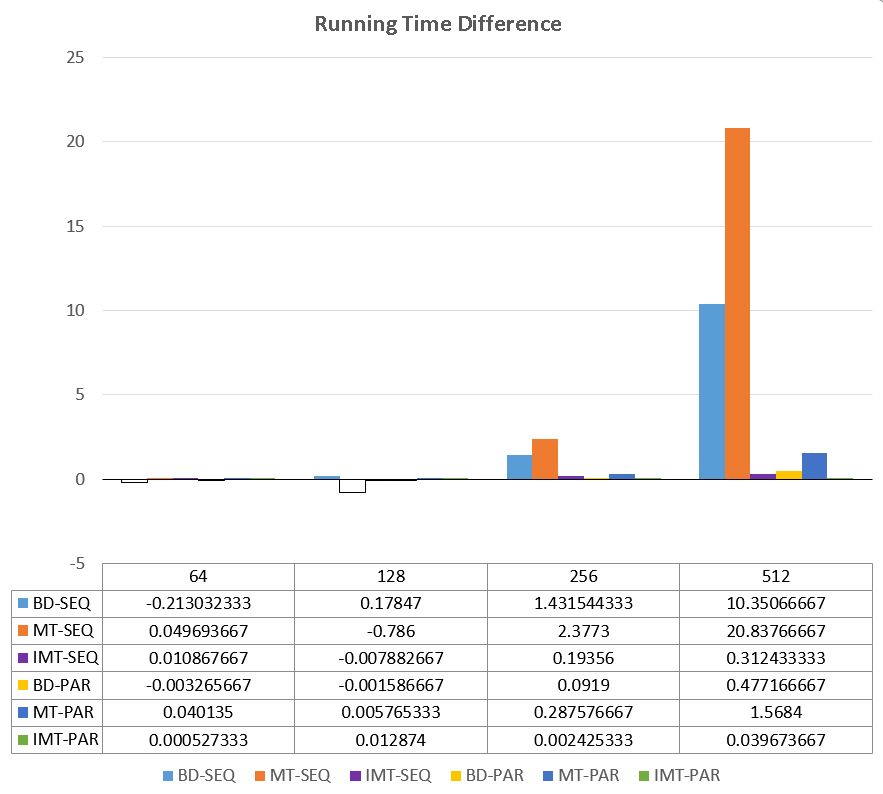
\includegraphics[height=.4\textheight
%  \includegraphics[width=\textwidth]{figures/results/runtime_diff.png}
%  \caption{The runtime difference between including the crowning computations or ignoring it. It is clear that the addition of the crowning module shows very little impact overall on the runtime, and the only cases where it impacts in a significant way are sequential runs.}
%  \label{fig:runtime_diff}
%\end{figure}
\begin{figure}%[!b]
\centering
  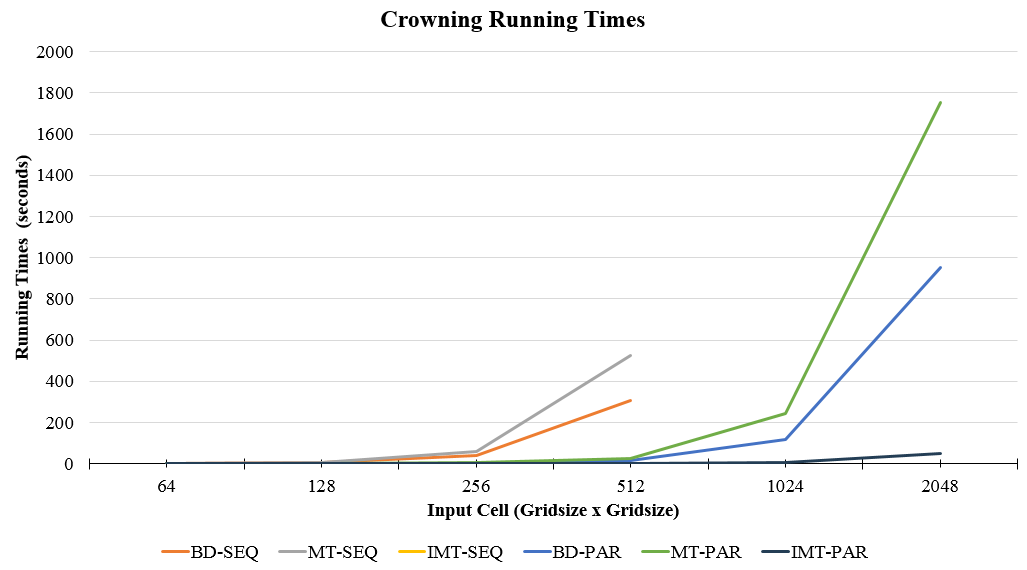
\includegraphics[width=\textwidth]{figures/results/crowning_reg.png}
  \caption{The runtimes to completion of simulation }
  \label{fig:runtimes}
\end{figure}  
\begin{figure}%[!b]
\centering
  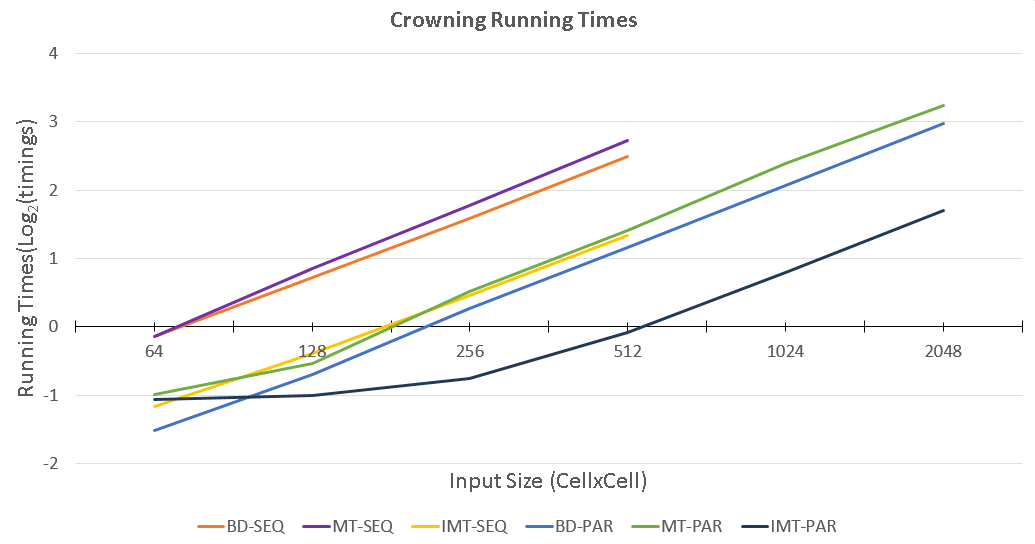
\includegraphics[width=\textwidth]{figures/results/crowning_log.png}
  \caption{The log-scale version of the graph found in Figure \ref{fig:runtimes}.}
  \label{fig:runtimes_log}
\end{figure} 

Take note that the runtimes for both the sequential and parallel versions of the IMT kernel take less time to run. The kernel does not require the use of atomic functions, and therefore runs much faster than the other kernels. The large simulation sizes were not tested for sequential due to the extreme amount of time they would require to compute. The kernels outperform their partner in the sequential implementation at almost all sizes for every kernel type. Notice that the final 2048x2048 grid simulation for the Burn Distances and Minimal Time Kernels are similar in runtimes to the 512x512 runtimes of their sequential counterparts. 

\subsection*{Throughput and Speedup}
Throughput is defined as the amount of data processed per unit time \cite{cuda}. This paper presents the throughput results for this paper in GigaBytes/Second. The throughput dividing the amount of data processed over the simulation by the amount of time it took to process that simulation. These results are displayed in $log_2$ scale for ease of comparison in Figure \ref{fig:throughput}.
\begin{figure}[H]
\centering
  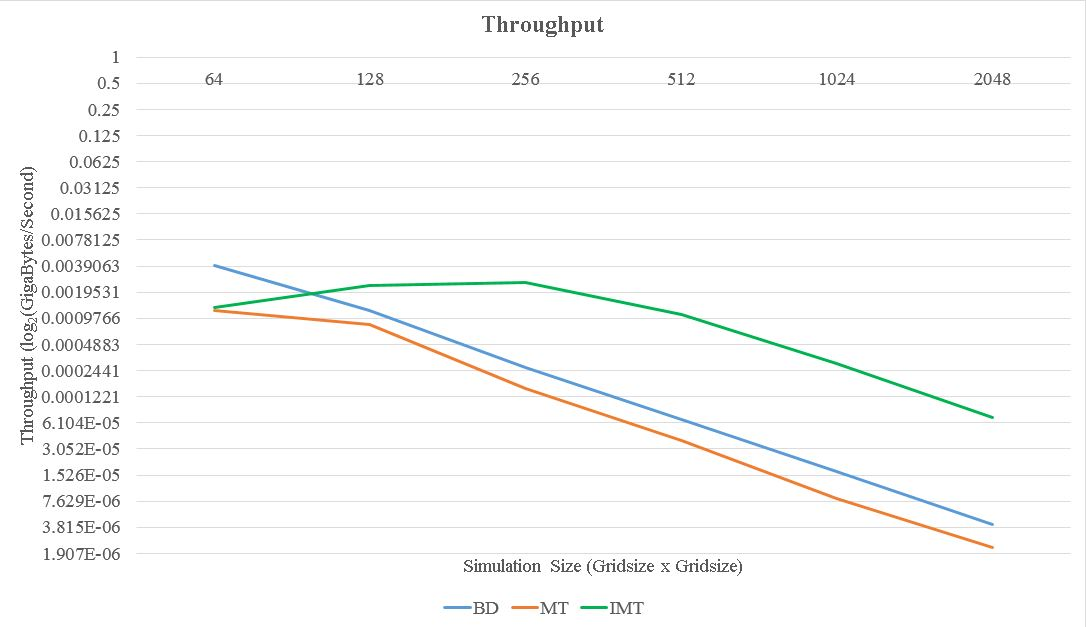
\includegraphics[width=\textwidth]{figures/results/throughput.JPG}
  \caption{The $log_2$ scale of the throughput results.}
  \label{fig:throughput}
\end{figure} 

The speedup is the amount that the parallel version is faster than the sequential version. This value is found by dividing the sequential running times by the parallel. These results can be seen in Figure \ref{fig:speedup}. 
\begin{figure}[H]
\centering
  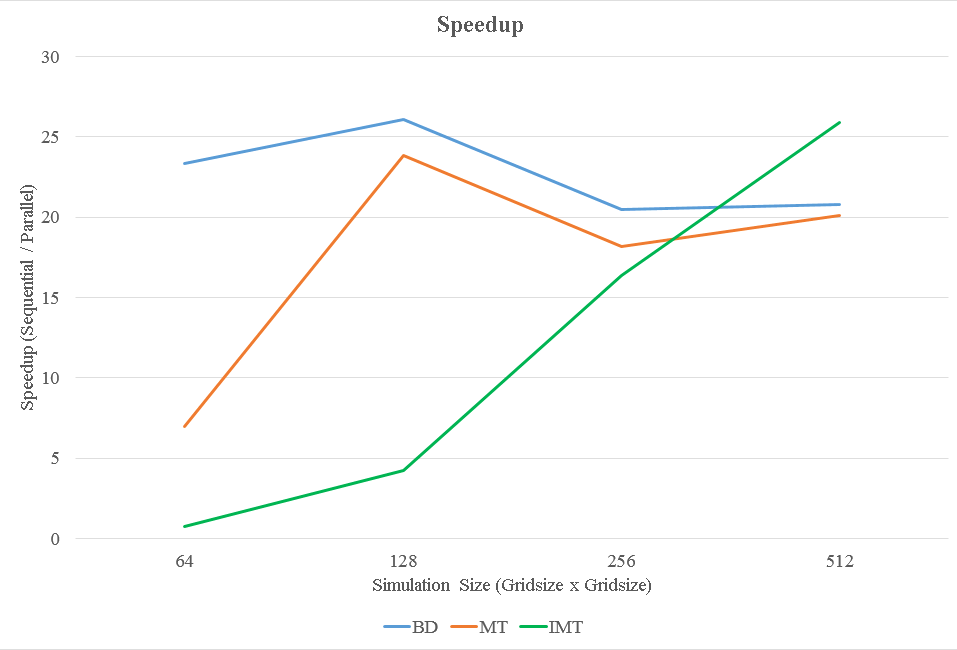
\includegraphics[width=\textwidth]{figures/results/speedup.png}
  \caption{The speedup between the parallel and sequential implementations. The average speedup was around 20X faster for all the versions.}
  \label{fig:speedup}
\end{figure} 

\subsection*{Memory Transfer Impact}
A major part of the time requirements for using CUDA is shipping the data from the host to the device \cite{cudabyexample}. In order to illustrate this time difference, the average running time with and without memory transfer was timed and may be seen in Figure \ref{fig:mem_comp}. Additionally, the average time it took to transfer memory per simulation size can be seen in Table \ref{table:mem_time}.
\begin{table}[H]
\centering
\caption{The average time to transfer memory from the CPU host to the GPU device in the three largest simulation sizes.}
\label{table:mem_time}
\begin{tabular}{l|c|}
\cline{2-2}
                           & \multicolumn{1}{l|}{Average Memory Transfer Time} \\ \hline
\multicolumn{1}{|l|}{512}  & 0.09242                                           \\ \hline
\multicolumn{1}{|l|}{1024} & 0.11389                                           \\ \hline
\multicolumn{1}{|l|}{2048} & 0.10288                                           \\ \hline
\end{tabular}
\end{table} 
\begin{figure}[H]
\centering
  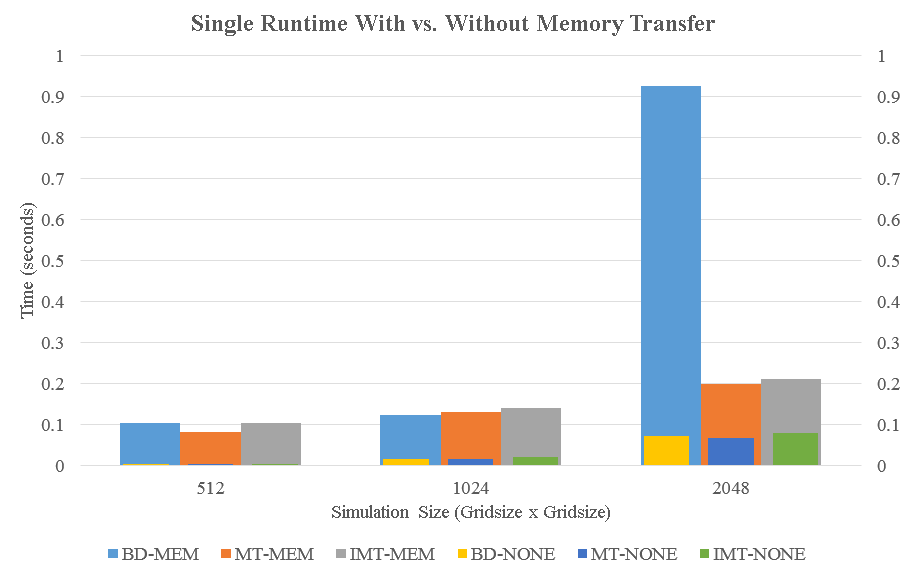
\includegraphics[height=.4\textheight]{figures/results/mem_compare.png}
  \caption{The runtimes found for a single iteration of the kernel call with and without memory transfer time.}
  \label{fig:mem_comp}
\end{figure} 
%\begin{figure}%[!b]
%\centering
% \includegraphics[width=\textwidth]
%{figures/results/memory_transfer.png}
%  \caption{This figure displays the average time it took to transfer the memory for each size, for all methods. The transfer of memory is roughly the same for each kernel.}
%  \label{fig:mem_trans}
%\end{figure} 

\subsection*{Simulation vs. Real Time}
This section presents the relationship between a real-world second and a simulation second. The library runs in faster-than-real-time, which means in a second of real-world time, the library can compute several seconds of simulation time data. The IMT kernel is fastest by far, which makes sense as it does not require any atomic functions to operate. Table \ref{table:time_comp} shows the comparisons for the three methods on two different input sizes on how they compare for simulation time versus real world time. 
\begin{table}[H]
\centering
\caption{A table containing the values for real-time versus simulation timesteps. Multiple simulation seconds are computed per real-world second.}
\label{table:time_comp}
\begin{tabular}{l|l|l|l|l|l|l|}
\cline{2-7}
                                                          & \multicolumn{3}{c|}{\cellcolor[HTML]{C0C0C0}\textbf{Size: 512}} & \multicolumn{3}{c|}{\cellcolor[HTML]{C0C0C0}\textbf{Size: 1024}} \\ \hline
\rowcolor[HTML]{EFEFEF} 
\multicolumn{1}{|l|}{\cellcolor[HTML]{EFEFEF}Kernel Used} & BD                  & MT                  & IMT                 & BD                 & MT                  & IMT                   \\ \hline
\multicolumn{1}{|l|}{Total Time Run (seconds)}            & 1                   & 1                   & 1                   & 3                  & 3                   & 3                     \\ \hline
\multicolumn{1}{|l|}{Total Iterations}                    & 240                 & 240                 & 220                 & 180                & 200                 & 180                   \\ \hline
\multicolumn{1}{|l|}{Max Time in Sim}                     & 477                 & 534                 & 6804                & 347                & 483                 & 7339                  \\ \hline
\multicolumn{1}{|l|}{Time / Iterations}                   & 1.99                & 2.22                & 30.93               & 1.98               & 2.415               & 40.77                 \\ \hline
\multicolumn{1}{|l|}{Real Time / Sim Time}                & 477                 & 534                 & 6804                & 119                & 161                 & 2446.33               \\ \hline
\end{tabular}
\end{table}

\subsection*{Wind}\label{sec:wind}
A brief example of the influence of wind is presented in this section. The two examples are found as follows, and include a wind direction in the positive x direction in Figure \ref{fig:wind} and both in the positive x and y in Figure \ref{fig:wind_both}. 
\begin{figure}[H]
\centering
  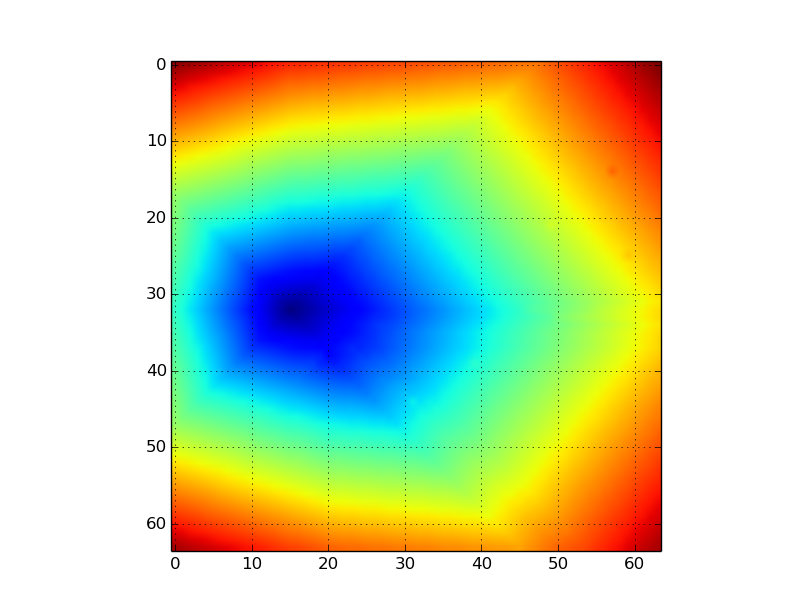
\includegraphics[height=.4\textheight]{figures/results/40_wind.png}
  \caption{Effect of the wind on a kernel when the wind is a value of 40 in the positive x direction.}
  \label{fig:wind}
\end{figure}  
\begin{figure}[H]
\centering
  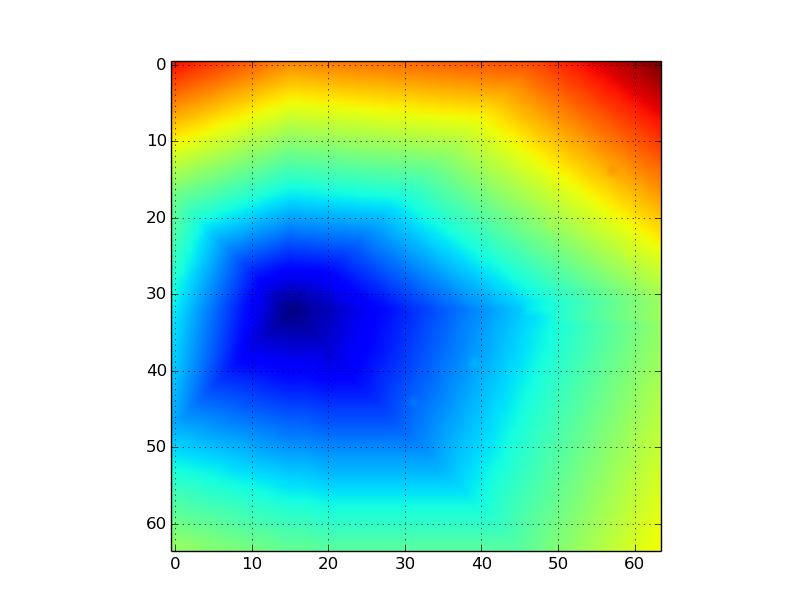
\includegraphics[height=.4\textheight]{figures/results/40_40_wind.png}
  \caption{Effect of the wind on a kernel when the wind is a value of 40 in the positive x and y direction.}
  \label{fig:wind_both}
\end{figure} 

\subsection*{Spotting}
Unfortunately, the data necessary to run a full-scale spotting test was unavailable. The implementation was performed as though the data was available, however several approximations had to be made. Every ember was assumed to launch to the same height, and then the descent was calculated from that point. The model described in the Implementation chapter was implemented as far as it could go, but for some prototype results, the following figures are presented. Wind is a requirement for spotting to occur, or the ember would be launched and just land back in the already-burning cell. The wind in Figure \ref{fig:spot_40} is in the x-direction only, while the wind in Figure \ref{fig:spot_40_20} is higher in the x, but has a value in the y direction as well. The windspeeds were chosen as to be comparable to those presented in Section \ref{sec:wind}.
\begin{figure}%[!b]
\centering
  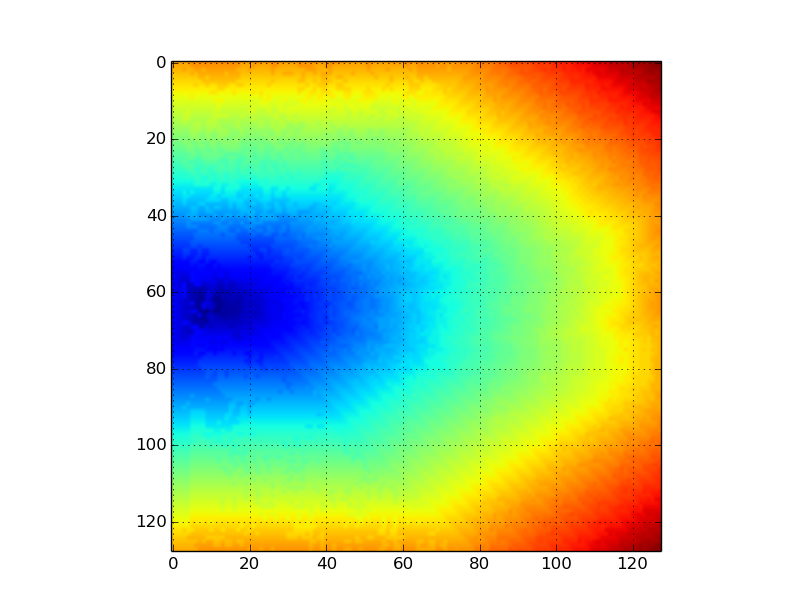
\includegraphics[height=.38\textheight]{figures/results/spot_40.png}
  \caption{The prototype results for the spotting module. The wind in this figure is gusting at a value of 40 in the x direction.}
  \label{fig:spot_40}
\end{figure}  
\begin{figure}%[!b]
\centering
  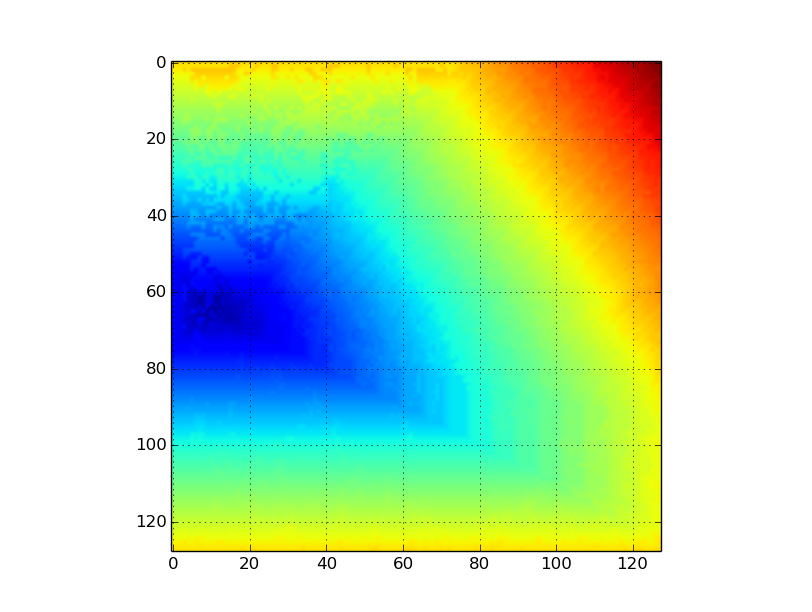
\includegraphics[height=.38\textheight]{figures/results/spot_40_40.png}
  \caption{The prototype results for the spotting module. The wind in this figure is gusting at a value of 40 in the x direction and 20 in the y direction.}
  \label{fig:spot_40_20}
\end{figure} 

\section{Kyle Canyon}
For the final set of tests, the Burn Distances kernel was run on the data for Kyle Canyon in southern Nevada. Only the BD kernel is shown here because all the outputs are very similar. This is an example of a real-world application of the simulator working. Kyle canyon's real-world data was input into the simulator, where a long-term simulation was run. The simulation was paused at three points to illustrate the gradual spread of the fire: Figure \ref{fig:kyle_5000} stopped after 5000 iterations (20.5 seconds to run), Figure \ref{fig:kyle_7000} stopped after 7000 iterations (28.8 seconds), and Figure \ref{fig:kyle_10000} stopped after 10,000 iterations (41.1 seconds). The scale at which the simulation was run meant each time step was equivalent to 100 seconds, as was found in vFire \cite{vFire}. The end time of the simulation was approximately 2.1 days after the beginning of the simulation. The three images are to give a comparison of what the progression of fire looks like. 
\begin{figure}[!b]
\centering
  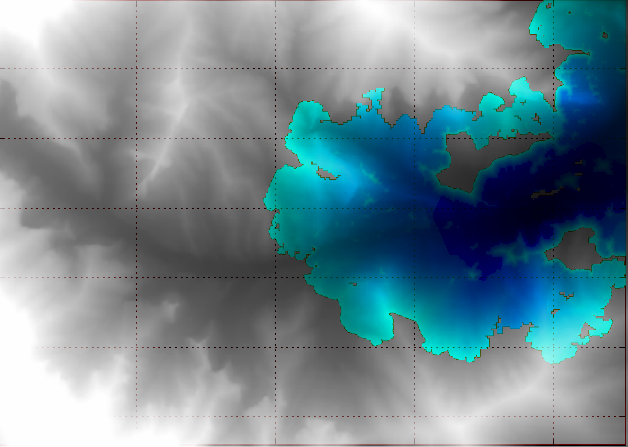
\includegraphics[height=.4\textheight]{figures/results/overlay_5.png}
  \caption{The Kyle Canyon fire started at the entrance to the canyon after 5000 iterations in simulation. This simulation is timestamped at approximately 0.68 days or 16.4 hours.}
  \label{fig:kyle_5000}
\end{figure}  
\begin{figure}%[!b]
\centering
  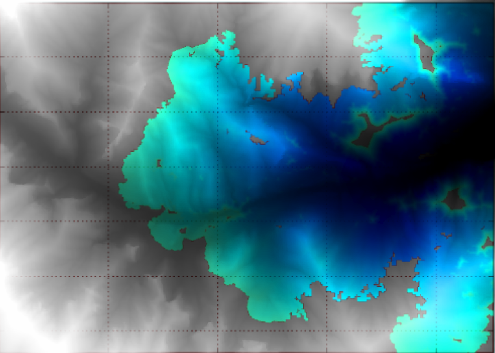
\includegraphics[height=.4\textheight]{figures/results/7000.png}
  \caption{The Kyle Canyon fire started at the entrance to the canyon after 7000 iterations in simulation. This simulation is timestamped at approximately 1.2 days.}
  \label{fig:kyle_7000}
\end{figure} 
\begin{figure}%[!b]
\centering
  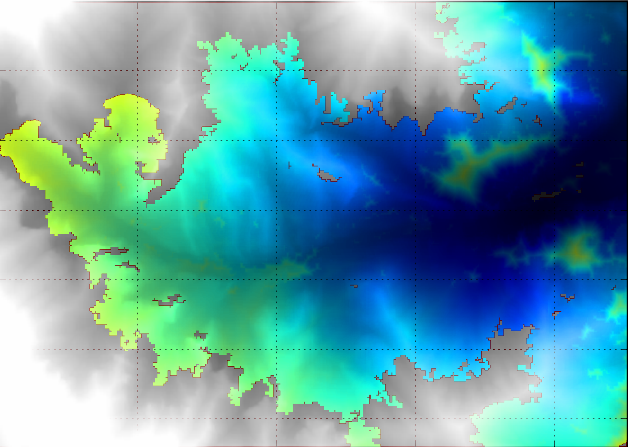
\includegraphics[height=.4\textheight]{figures/results/overlay_7.png}
  \caption{The Kyle Canyon fire started at the entrance to the canyon after 10,000 iterations in simulation. This simulation is timestamped at approximately 2.1 days.}
  \label{fig:kyle_10000}
\end{figure} 

This thesis presented several avenues for results, including a base spread, running times, throughput comparisons, speedup comparisons, and real-world simulation data. The simulation runs in reasonable time on real-world data, and all three kernels achieved approximately 20X speedup. While the work accomplished in this paper is a good start, there are still areas where improvements and additions can be made. 

